
%===================================================================================
% Chapter: Introduction
%===================================================================================
\chapter{Propuesta}\label{chapter:propuesta}
%===================================================================================
Se propone un sistema para la generación de texto alternativo a partir de las imágenes del repositorio digital del patrimonio cultural de la Oficina del Historiador, combinando múltiples modelos de aprendizaje profundo. La metodología se basa en un enfoque de evaluación comparativa entre diferentes modelos de generación de texto a partir de imágenes, utilizando un criterio de selección basado en la similitud semántica con el contenido visual.

En primer lugar, se emplea el modelo BLIP (Bootstrapped Language-Image Pretraining) para generar una primera descripción de la imagen. Posteriormente, la imagen es procesada por el modelo ViT (Vision Transformer) en conjunto con GPT-2, obteniendo una segunda descripción independiente. Finalmente, el modelo CLIP (Contrastive Language-Image Pretraining) se utiliza como mecanismo de selección, comparando las dos descripciones generadas y eligiendo la que presente una mayor correspondencia semántica con la imagen de entrada.

% TODO: \usepackage{graphicx} required
\begin{figure}
	\centering
	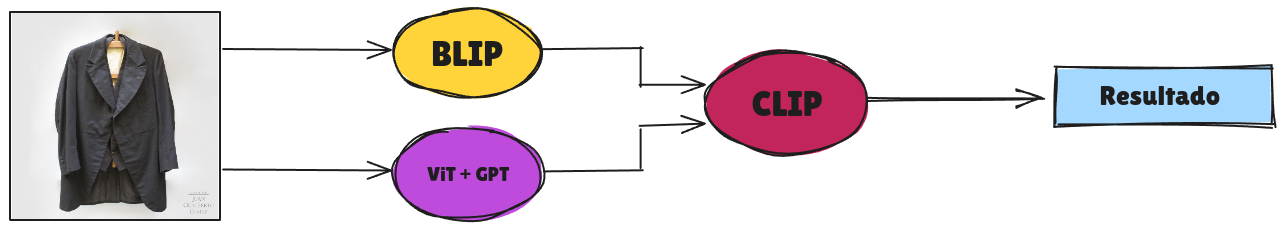
\includegraphics[width=1\linewidth]{./Graphics/diagrama}
	\caption{Modelo general}
	\label{fig:diagrama}
\end{figure}
